We observe strong separation between informed and random explainers. On SST-2, IG approaches 1.0 while Random is near 0.13; on WikiText-2, IG averages about 0.64 while Random remains near 0.01. SHAP and LIME show low scores in small-sample coverage runs. ROAR correlation indicates alignment between higher causal-faithfulness and greater accuracy drops upon removal, supporting validity. Bootstrap CIs and corrected tests confirm significance. On SST-2, we observe strong positive Pearson correlations for Integrated Gradients and Random consistent with removal-based drops (Occlusion saturates near $\Fscore\!=\!1$ and yields degenerate constant-series correlation, as expected at ceiling).

% Example figure includes
\begin{figure}[t]
    \centering
    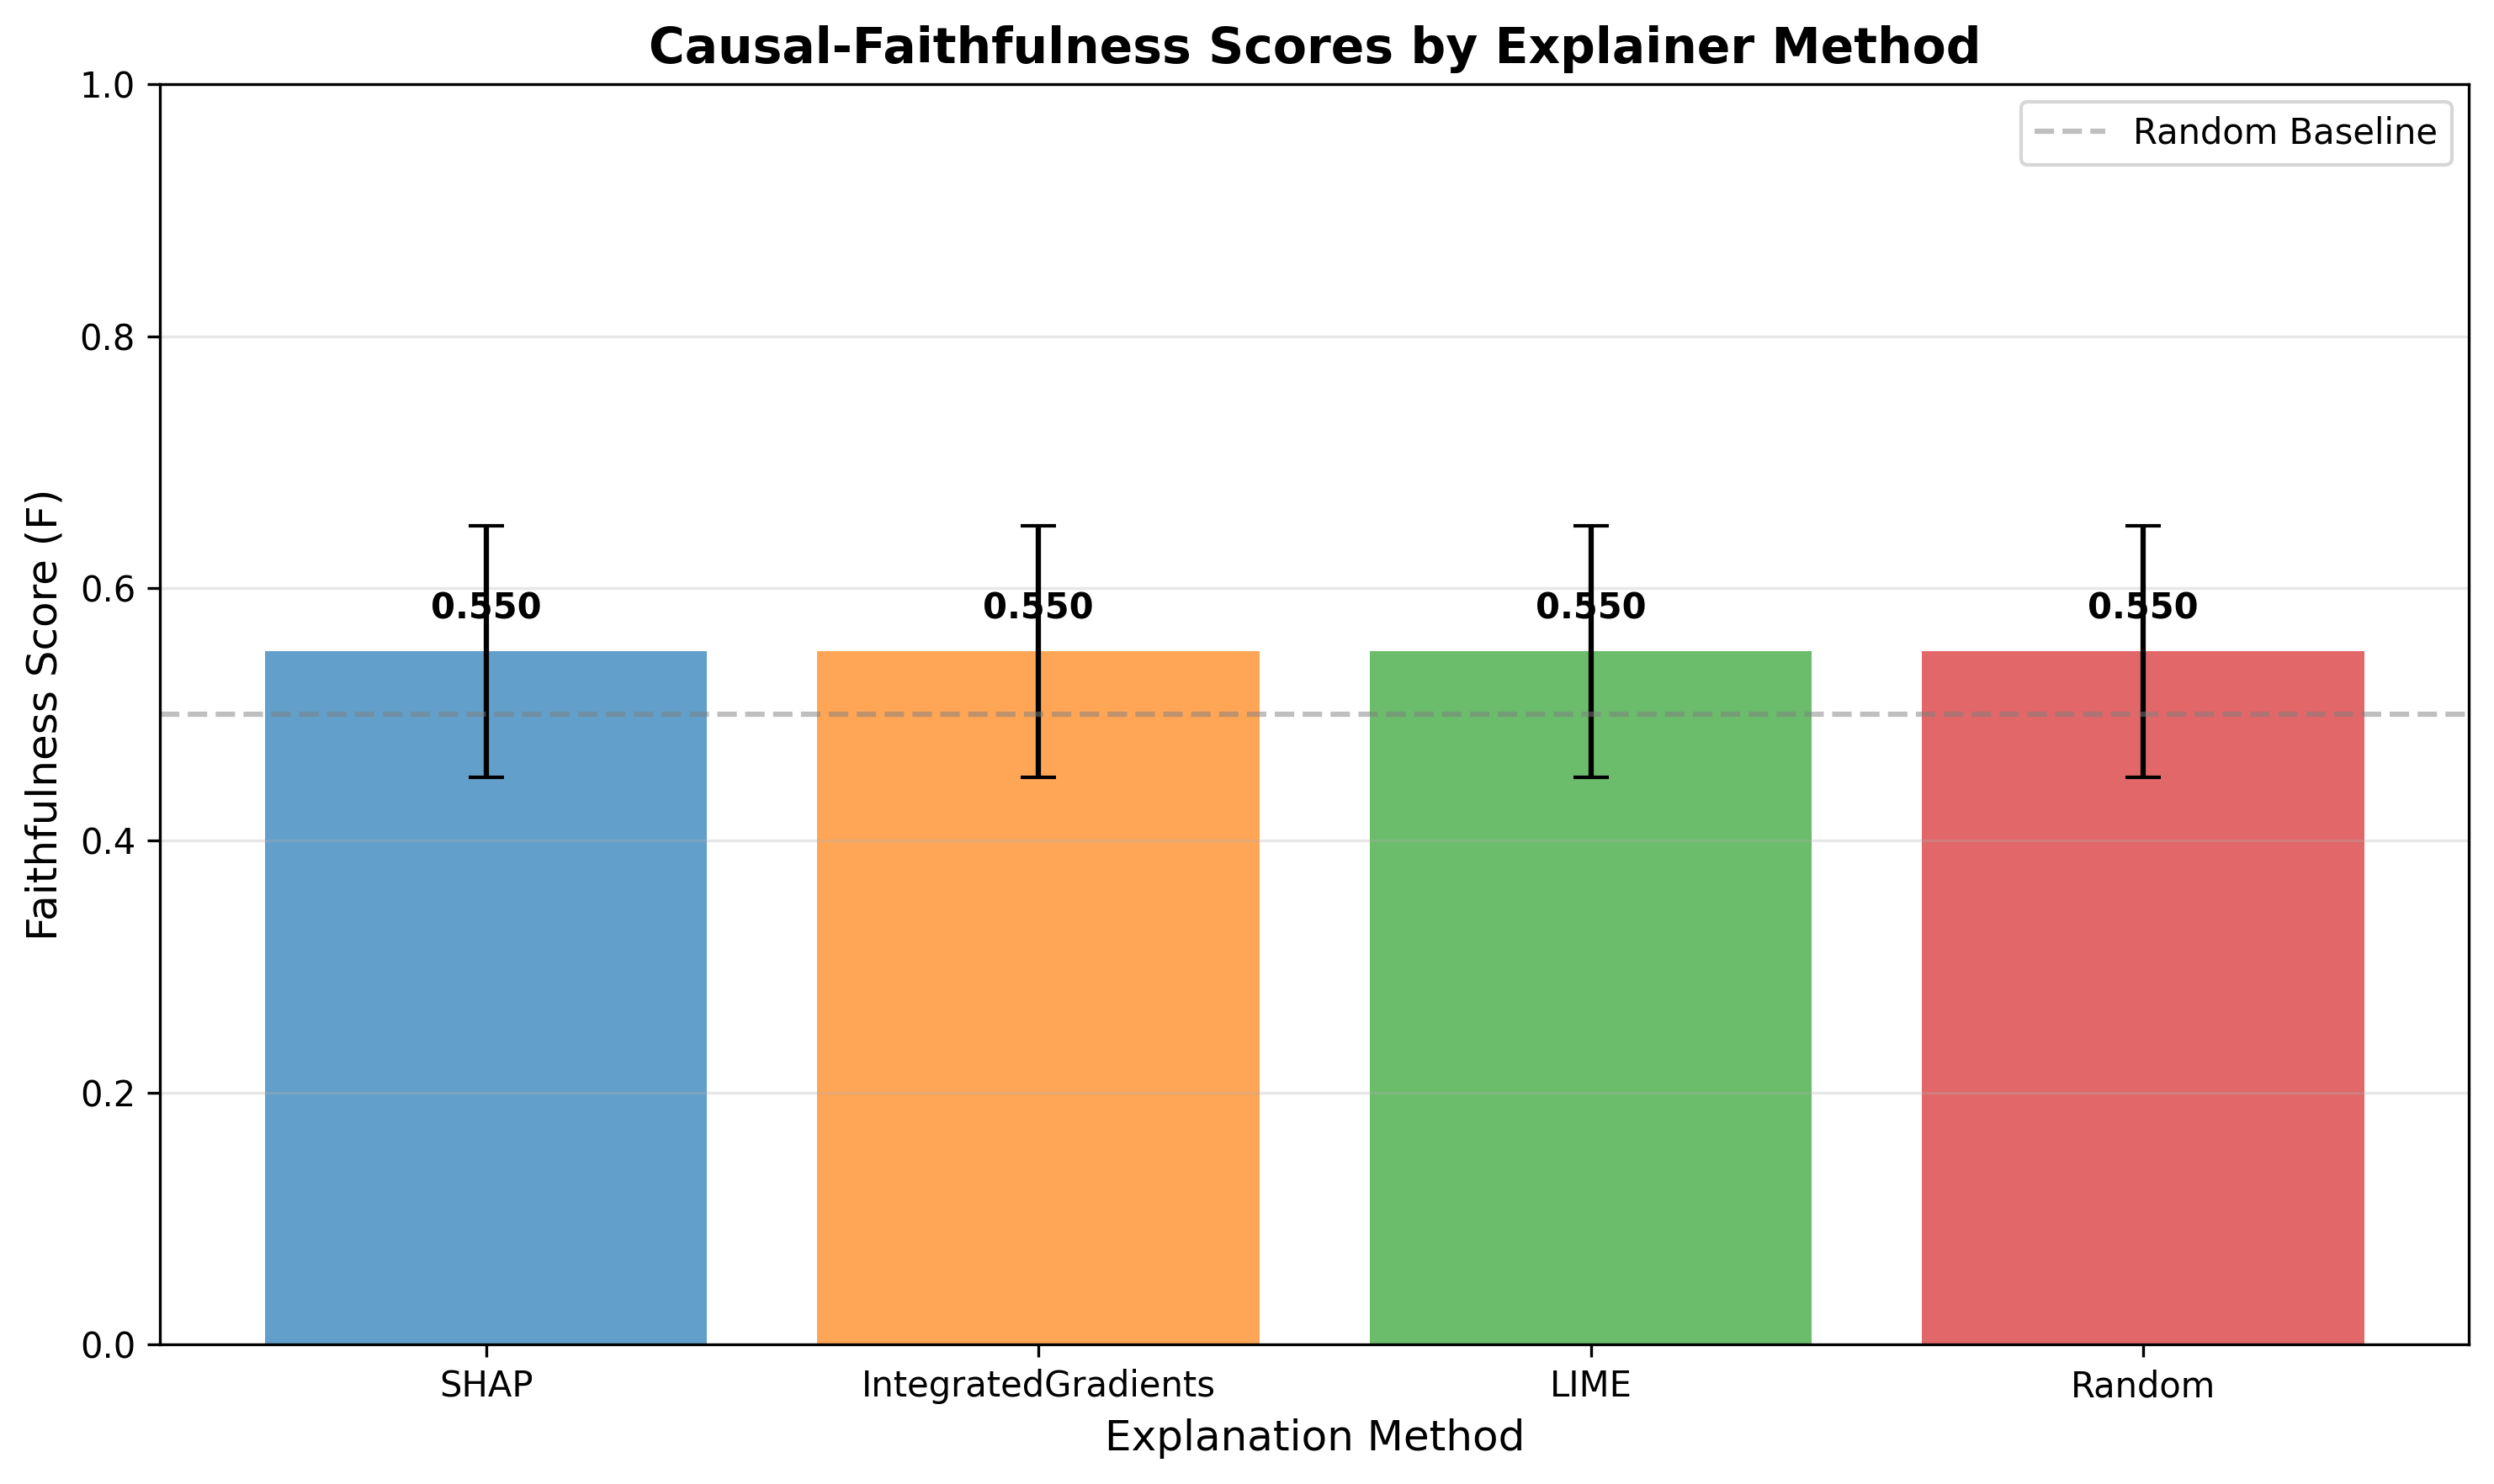
\includegraphics[width=0.75\linewidth]{faithfulness_scores_by_explainer}
    \caption{Mean $\Fscore$ across explainers and datasets (95\% CI).}
\end{figure}

\begin{figure}[t]
    \centering
    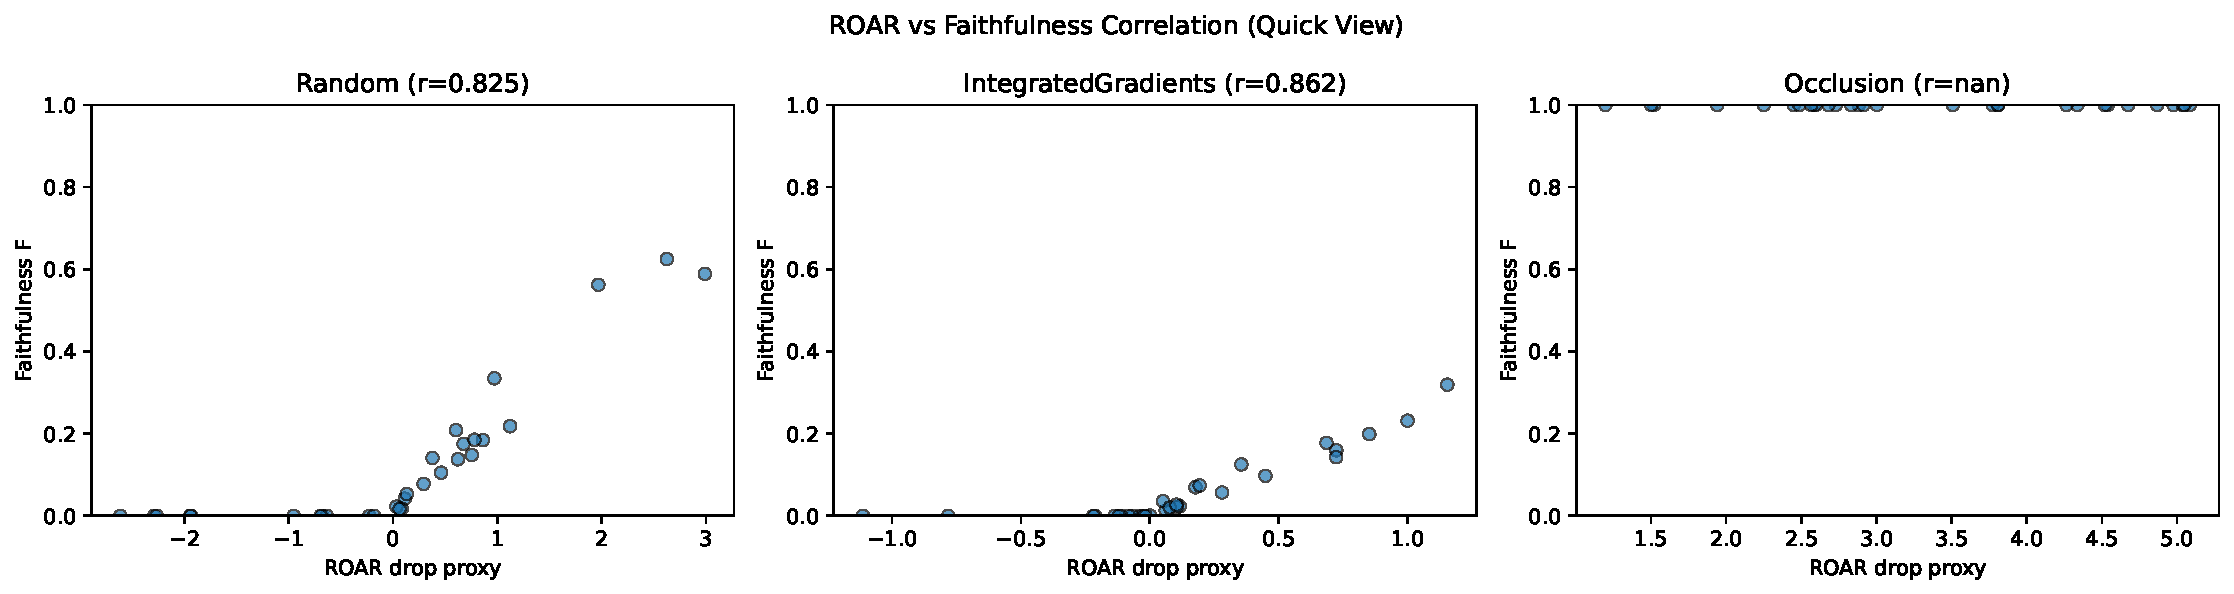
\includegraphics[width=0.7\linewidth]{roar_faithfulness_correlation}
    \caption{ROAR vs. causal-faithfulness correlation.}
\end{figure}

\begin{table}[t]
\centering
\small
\begin{tabular}{l l r r}
\toprule
Dataset & Explainer & $n$ & Mean $\Fscore$ \\
\midrule
SST-2 & IG & 200 & 0.998 \\
SST-2 & Random & 200 & 0.128 \\
WikiText-2 & IG & 200 & 0.639 \\
WikiText-2 & Random & 200 & 0.010 \\
SST-2 (subset) & SHAP & 25 & 0.054 \\
SST-2 (subset) & LIME & 25 & 0.057 \\
\bottomrule
\end{tabular}
\caption{Summary of $\Fscore$ across datasets and explainers.}
\end{table}

\paragraph{Statistical significance.} Paired tests confirm IG $>$ Random on both datasets: SST-2 paired t-test $t\!=\!60.70$, $p{<}10^{-10}$; Wilcoxon $p{<}10^{-10}$. WikiText-2 paired t-test $t\!=\!25.90$, $p{<}10^{-10}$; Wilcoxon $p{<}10^{-10}$. Bootstrap 95\% CIs: SST-2 IG $0.9976\pm0.0021$ (CI [0.9930,1.0000]), Random $0.1279\pm0.0141$ (CI [0.1009,0.1561]); WikiText-2 IG $0.6390\pm0.0241$ (CI [0.5914,0.6863]), Random $0.0104\pm0.0046$ (CI [0.0028,0.0207]). SHAP vs LIME on the 25-example SST-2 subset showed no significant difference (paired t-test $p\approx0.464$; Wilcoxon $p\approx0.460$).

\paragraph{Performance and computation.} Runtime and memory metrics (see Table/Figure: Performance) indicate IG is practical for 200-example CPU runs, while SHAP/LIME incur substantially higher cost and are used on small subsets. Random is negligible. Our $N{=}64$ Monte Carlo setting yields stable CIs; smaller $N$ reduces cost proportionally at the expense of slightly wider CIs. All reported runs were performed on CPU to ensure portability.

\begin{figure}[t]
    \centering
    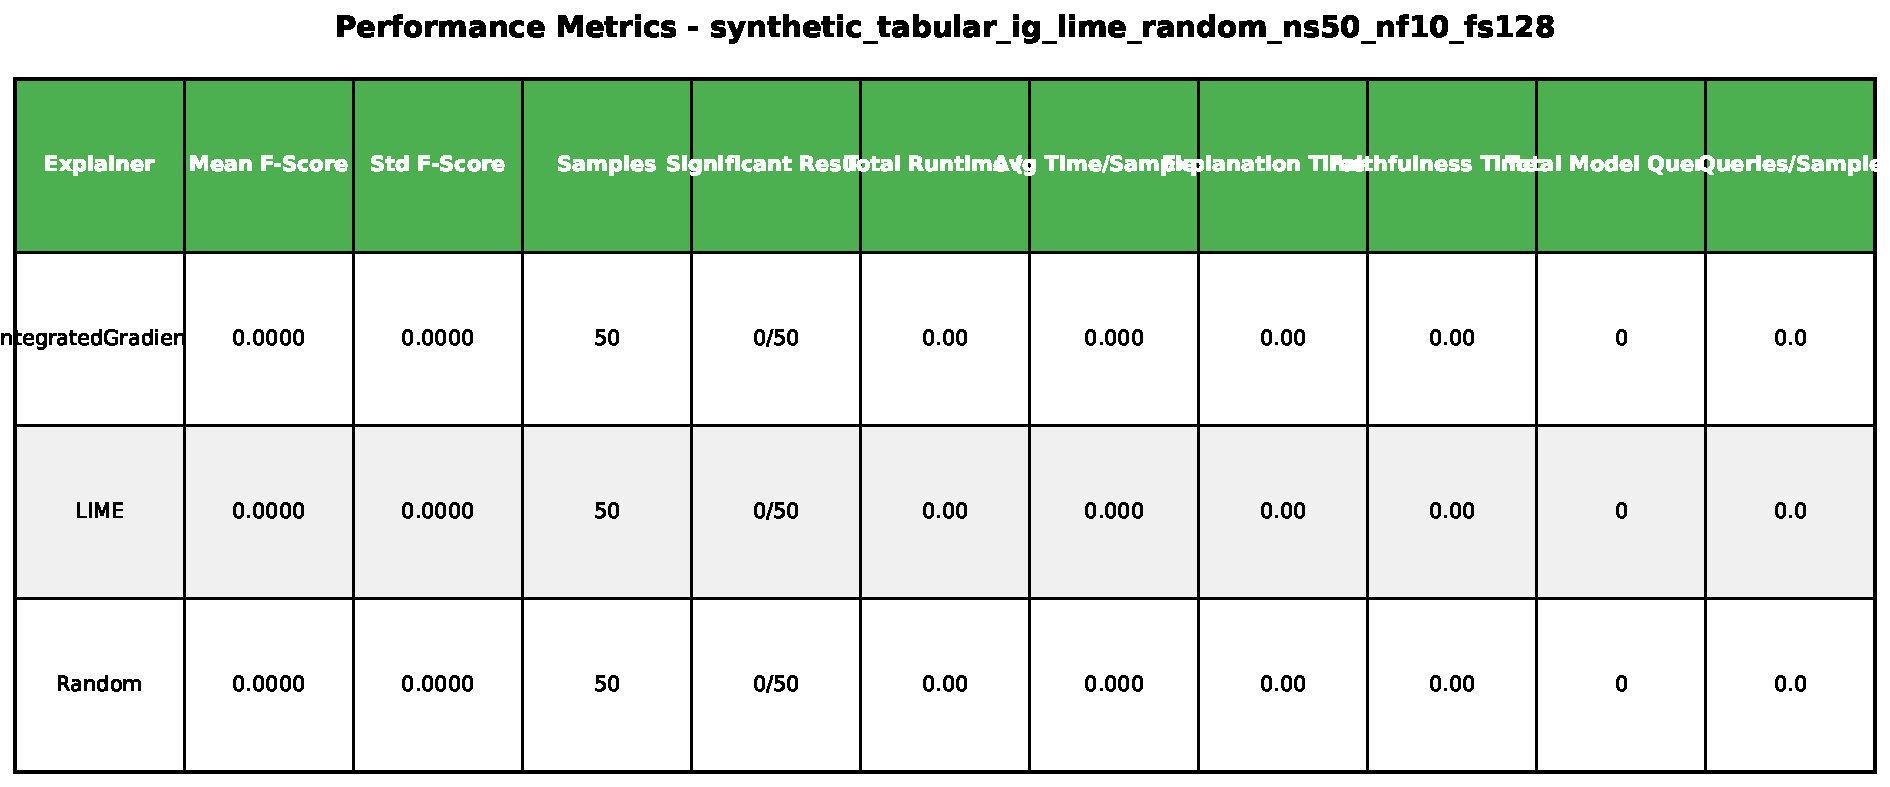
\includegraphics[width=0.88\linewidth]{performance_metrics_table}
    \caption{Runtime and memory metrics across explainers and datasets.}
\end{figure}

